\documentclass{article}
\usepackage[utf8]{inputenc}
\usepackage[T1]{fontenc}
\usepackage[margin=0.75in]{geometry}
\usepackage{amsmath, amssymb, amsfonts}
\usepackage{pgfplots}
\usepackage{tikz}
\usepackage{booktabs}
\usetikzlibrary{patterns, arrows.meta, backgrounds}
\usepgfplotslibrary{fillbetween}
\pgfplotsset{compat=1.18}

% --- Colors & Styles ---
\definecolor{trueColor}{RGB}{50, 150, 200}   % Blue/Teal for TP, TN
\definecolor{falseColor}{RGB}{200, 80, 80}   % Red for FP, FN
\definecolor{axisGrey}{RGB}{80, 80, 80}

\title{Sampled vs Simulated $p$-values uncertainty}
\date{}

% --- Macros ---
\newcommand{\N}{\ensuremath{\mathrm{N}}}
\newcommand{\PP}{\ensuremath{\mathrm{PP}}}
\newcommand{\PN}{\ensuremath{\mathrm{PN}}}
\newcommand{\TP}{\ensuremath{\mathrm{TP}}}
\newcommand{\TN}{\ensuremath{\mathrm{TN}}}
\newcommand{\FP}{\ensuremath{\mathrm{FP}}}
\newcommand{\FN}{\ensuremath{\mathrm{FN}}}
\newcommand{\PPR}{\ensuremath{\mathrm{PPR}}}

\begin{document}
% \maketitle

\section*{Definitions}
\begin{align*}
  \text{P} & = \text{Positive outcomes} = \FN + \TP           \\[0.5em]
  \N       & = \text{Negative outcomes} = \FP + \TN           \\[0.5em]
  \PP      & = \text{Predicted Positive outcomes} = \FP + \TP \\[0.5em]
  \PN      & = \text{Predicted Negative outcomes} = \FN + \TN
\end{align*}

\textbf{Positive Prediction Rate (PPR):}
\begin{align*}
  \PPR & = \frac{\PP}{\PP+\PN} = \frac{\TP + \FP}{\TP + \FN + \FP + \TN}
  = \frac{\TP + \FP}{\text{P} + \text{N}}
\end{align*}

\section*{Sampled $p$-value distribution}

$p$-value distribution classified as ``Predicted Positive'' (PP) when below $\alpha$ and ``Predicted Negative'' (PN) otherwise. Standard deviation ($\sigma_p$) is sampled from the distribution.

\vspace{1em}

\noindent

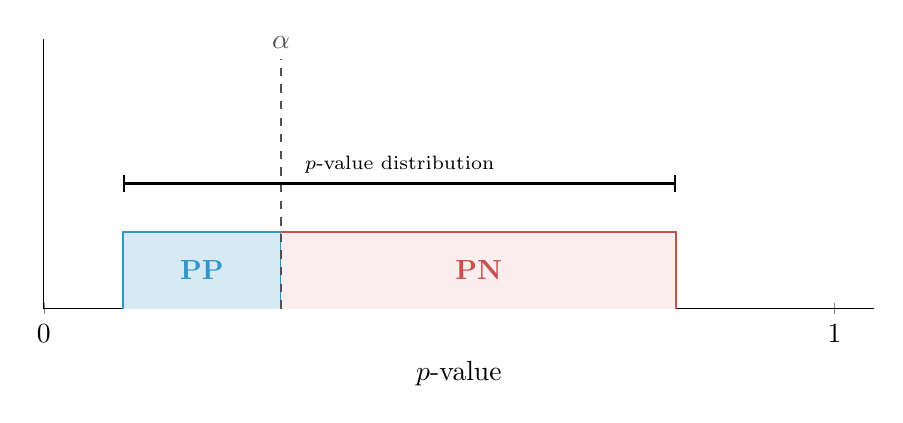
\begin{tikzpicture}
  \begin{axis}[
      axis lines=left,
      axis line style={-},
      xmin=0, xmax=1.05,
      ymin=0, ymax=1.4,
      xlabel={$p$-value},
      ytick=\empty,
      xtick={0,1},
      xticklabels={$0$,$1$},
      width=\linewidth, height=5cm,
      clip=false
    ]


    % --- Simplified Distributions ---
    % Region P (Positives)
    \fill[trueColor!20] (axis cs:0.1,0) rectangle (axis cs:0.3, 0.4);
    \draw[thick, trueColor] (axis cs:0.1,0) -- (axis cs:0.1,0.4) -- (axis cs:0.3,0.4) -- (axis cs:0.3,0);
    \node[trueColor] at (axis cs:0.2, 0.2) {\textbf{PP}};

    % Region N (Negatives)
    \fill[falseColor!10] (axis cs:0.3,0) rectangle (axis cs:0.8, 0.4);
    \draw[thick, falseColor] (axis cs:0.3,0.4) -- (axis cs:0.8,0.4) -- (axis cs:0.8,0);
    \node[falseColor] at (axis cs:0.55, 0.2) {\textbf{PN}};

    % Alpha line
    \draw[dashed, axisGrey] (axis cs:0.3,0) -- (axis cs:0.3,1.3);
    \node[above, axisGrey] at (axis cs:0.3,1.3) {$\alpha$};

    % Rejection Region Indicator
    \draw[|-|, thick] (axis cs:0.1,0.65) -- (axis cs:0.8,0.65)
    node[midway, above, font=\scriptsize] {$p$-value distribution};

  \end{axis}
\end{tikzpicture}

\section*{Simulated $p$-value using Beta distributions}

Standard deviation $\sigma_p$ is simulated using uncertainty formulae from Table~\ref{tab:stat_uncertainty}. Uncertainty on $p$-value is modeled using Beta distributions. With $\mathbb{E}[\beta] = p_0$ and $\mathrm{Var}[\beta] = \sigma_p^2$, we solve for parameters $a, b$:
\[
  \begin{cases}
    p_0 = \frac{a}{a+b} \\
    \sigma_p^2 = \frac{ab}{(a+b)^2 (a+b+1)}
  \end{cases}
  \implies
  \begin{cases}
    a = p_0 \left( \frac{p_0 (1 - p_0)}{\sigma_p^2} - 1 \right) \\
    b = (1 - p_0) \left( \frac{p_0 (1 - p_0)}{\sigma_p^2} - 1 \right)
  \end{cases}
\]

Then, we have two cases depending on $p_0$ significance:

\vspace{1em}

% --- H1 Figure (Positive) ---
\noindent
\begin{minipage}[t]{0.48\textwidth}
  \centering
  \textbf{Negative Case} \\

  \vspace{0.5em}

  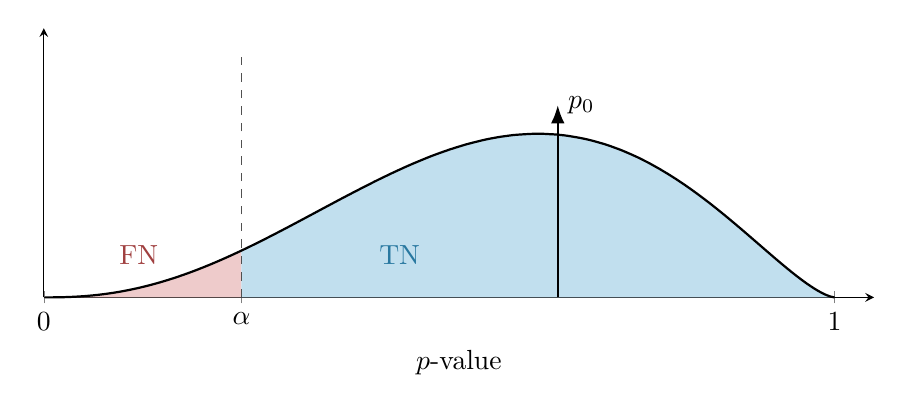
\begin{tikzpicture}
    \begin{axis}[
        axis lines=left,
        xmin=0, xmax=1.05,
        ymin=0, ymax=3.5,
        xlabel={$p$-value},
        ytick=\empty,
        xtick={0,0.25,1},
        xticklabels={$0$,$\alpha$,$1$},
        width=\linewidth, height=5cm,
        clip=false
      ]

      % Beta Distribution Curve for H1 (Skewed Left: a=1.5, b=6)
      % Approx function for visualization
      \addplot[thick, samples=200, domain=0.001:1, name path=H1Curve]
      {30 * x^(2.5) * (1-x)^1.5};

      \path[name path=xaxis] (axis cs:0,0) -- (axis cs:1,0);

      % Alpha line
      \draw[dashed, axisGrey] (axis cs:0.25,0) -- (axis cs:0.25,3.2);

      % --- Shading ---
      % FP (Type I Error): [0, alpha]
      \addplot[falseColor!30] fill between[of=H1Curve and xaxis, soft clip={domain=0:0.25}];
      % TN (Correct): (alpha, 1]
      \addplot[trueColor!30] fill between[of=H1Curve and xaxis, soft clip={domain=0.25:1}];

      % Labels
      \node[falseColor!80!black] at (axis cs:0.12, 0.55) {\textbf{\FN}};
      \node[trueColor!80!black] at (axis cs:0.45, 0.55) {\textbf{\TN}};

      % Sample p0
      \draw[-{Latex}, thick] (axis cs:0.65, 0) -- (axis cs:0.65, 2.5) node[above, right] {$p_0$};

    \end{axis}
  \end{tikzpicture}
  \begin{align*}
    \mathbb{P}[\FN] & = \int_0^\alpha \beta(x; a, b) dx \\
    \mathbb{P}[\TN] & = 1 - \mathbb{P}[\FN]
  \end{align*}
\end{minipage}%
\hfill
% --- H0 Figure (Negative) ---
\begin{minipage}[t]{0.48\textwidth}
  \centering
  \textbf{Positive Case} \\

  \vspace{0.5em}

  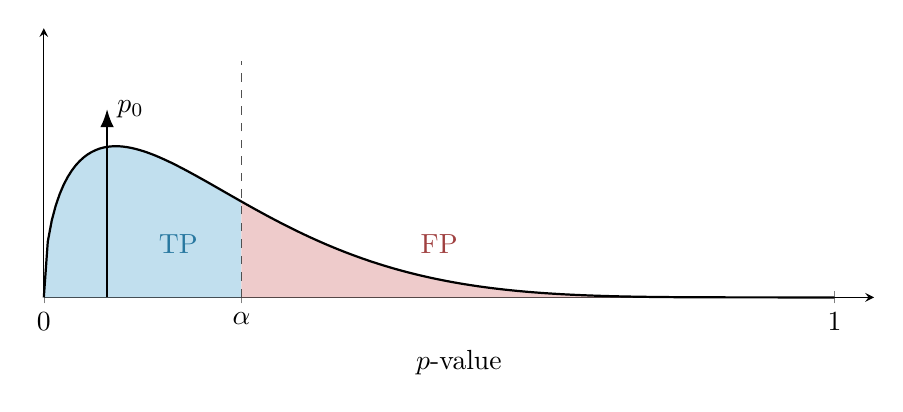
\begin{tikzpicture}
    \begin{axis}[
        axis lines=left,
        xmin=0, xmax=1.05,
        ymin=0, ymax=2.5,
        xlabel={$p$-value},
        ytick=\empty,
        xtick={0,0.25,1},
        xticklabels={$0$,$\alpha$,$1$},
        width=\linewidth, height=5cm,
        clip=false
      ]

      % Beta Distribution Curve for H0 (Skewed Right: a=4, b=1.5)
      % Approx function: x^(3) * (1-x)^(0.5) scaled
      \addplot[thick, samples=200, domain=0:1, name path=H0Curve]
      {7.5 * x^(0.5) * (1-x)^(5)};

      \path[name path=xaxis] (axis cs:0,0) -- (axis cs:1,0);

      % Alpha line
      \draw[dashed, axisGrey] (axis cs:0.25,0) -- (axis cs:0.25,2.2);

      % --- Shading ---
      % TP (Correct): [0, alpha]

      \addplot[trueColor!30] fill between[of=H0Curve and xaxis, soft clip={domain=0:0.25}];
      % FN (Type II Error): (alpha, 1]
      \addplot[falseColor!30] fill between[of=H0Curve and xaxis, soft clip={domain=0.25:1}];

      % Labels
      \node[trueColor!80!black] at (axis cs:0.17, 0.5) {\textbf{\TP}};
      \node[falseColor!80!black] at (axis cs:0.5, 0.5) {\textbf{\FP}};

      % Sample p0
      \draw[-{Latex}, thick] (axis cs:0.08, 0) -- (axis cs:0.08, 1.75) node[above, right] {$p_0$};

    \end{axis}
  \end{tikzpicture}
  \begin{align*}
    \mathbb{P}[\TP] & = \int_0^\alpha \beta(x; a, b) dx \\
    \mathbb{P}[\FP] & = 1 - \mathbb{P}[\TP]
  \end{align*}
\end{minipage}


\begin{table}[ht]
  \centering
  \begin{tabular}{lll}
    \toprule
    \textbf{Statistic}
                        & \textbf{Numerical standard deviation}
                        & \textbf{Numerical p-value uncertainty}                                                                                                           \\
    \midrule
    Cohen's $d$         & $\sigma_d \approx\nu_{\mathrm{npv}}\frac{2}{\sqrt{n}}$             & \multicolumn{1}{c}{-}                                                       \\
    Two-sample $t$      & $\sigma_t \approx \nu_{\mathrm{npv}}        $                      & $\sigma_{p} \approx 2f_{t,df}(|t|)\nu_{\mathrm{npv}}$                       \\
    Partial correlation & $\sigma_r \geq \nu_{\mathrm{npv}}\sqrt{\frac{(1-r^{2})^{3}}{n-1}}$ & $\sigma_{p} \geq 2f_{t,df}(|t|)\sqrt{\frac{df}{n-1}}\nu_{\mathrm{npv}}$     \\
    ANCOVA              & $\sigma_F \approx 2\sqrt{F}\nu_{\mathrm{npv}}$                     & $\sigma_{p} \approx 2\sqrt{F}f_{\mathcal{F}}(F;1,df_2)\,\nu_{\mathrm{npv}}$ \\
    \bottomrule
  \end{tabular}
  \caption{First-order numerical uncertainty of common statistical tests under
    Monte Carlo Arithmetic perturbations. Cohen's d formula assumes large
    and equal group sizes. $f_{t,df}$ and $f_\mathcal{F}(F;1,df_2)$ denote
    the probability density functions of the Student's $t$-distribution with
    $df$ degrees of freedom and the $\mathcal{F}$-distribution with $(1,
      df_2)$ degrees of freedom, respectively. The $p$-value approximation for
    the partial correlation uses $t=r(df/(1-r^2))^{1/2}$.}
  \label{tab:stat_uncertainty}
\end{table}

\end{document}